\section{Formal analysis using alloy}
\label{sect:formalanalysisusingalloy}

\subsection{Alloy code}
\label{subsect:alloycode}

For the evaluation of the model and the elicitation of the requirements we used the specification language Alloy which enabled us to express the structural and behavioral constraints of the software system.

\alloyfile{Files/alloy.als}

\subsection{Alloy results}
\label{subsect:alloyresults}

The following images are the results of the execution of the checks.

\begin{figure}[h!]
    \centering
    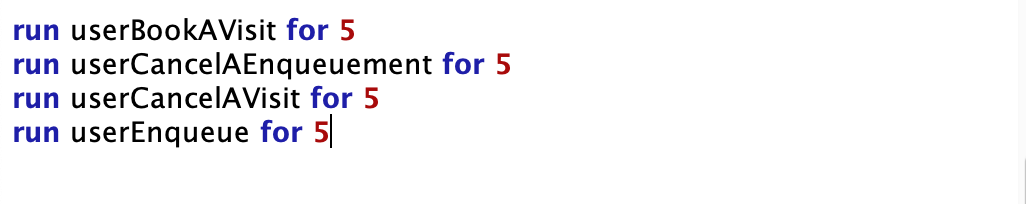
\includegraphics[width=0.6\textwidth]{Images/alloy/runs.png}
    \caption{\label{fig:runs}{todo}}
\end{figure}

\begin{figure}[h!]
    \centering
    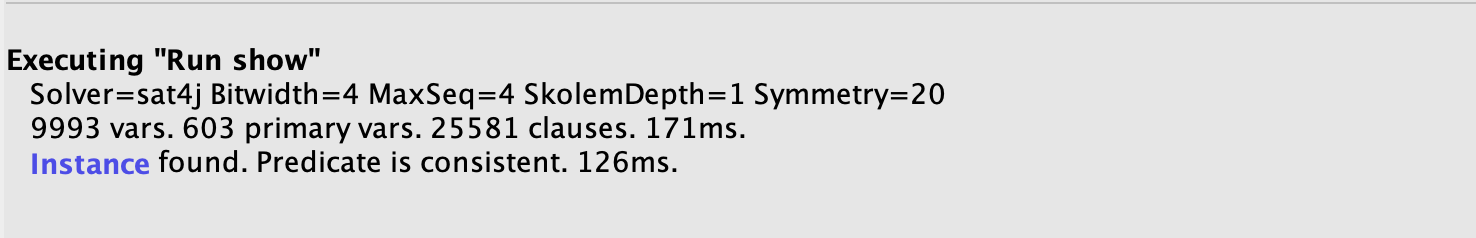
\includegraphics[width=0.6\textwidth]{Images/alloy/runshow.png}
    \caption{\label{fig:runshow}{todo}}
\end{figure}

\begin{figure}[h!]
    \centering
    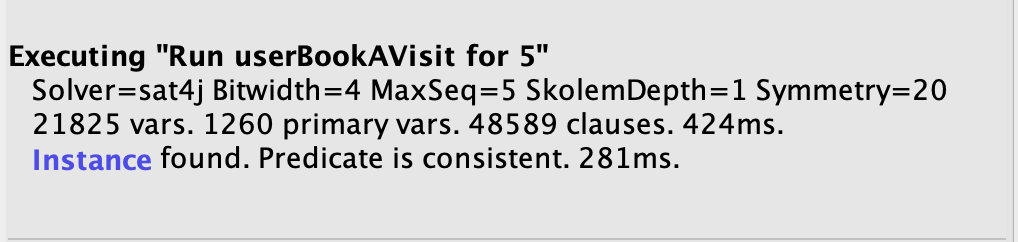
\includegraphics[width=0.6\textwidth]{Images/alloy/userbooksavisit.png}
    \caption{\label{fig:userbooksavisitalloy}{todo}}
\end{figure}

\begin{figure}[h!]
    \centering
    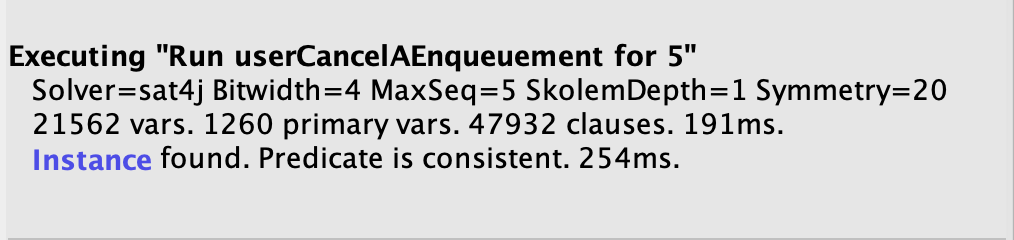
\includegraphics[width=0.6\textwidth]{Images/alloy/usercancelsanenqueuement.png}
    \caption{\label{fig:usercancelsanenqueuementalloy}{todo}}
\end{figure}

\begin{figure}[h!]
    \centering
    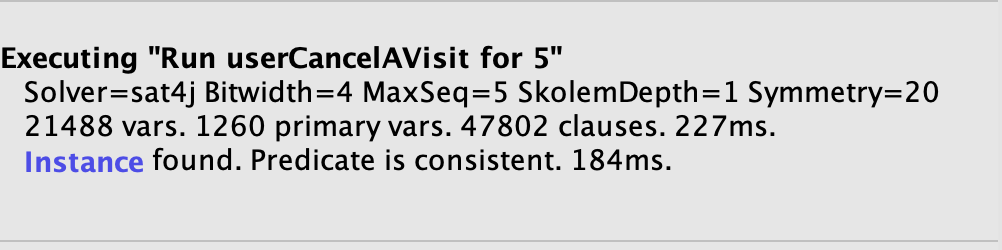
\includegraphics[width=0.6\textwidth]{Images/alloy/usercancelsavisit.png}
    \caption{\label{fig:usercancelsavisitalloy}{todo}}
\end{figure}

\begin{figure}[h!]
    \centering
    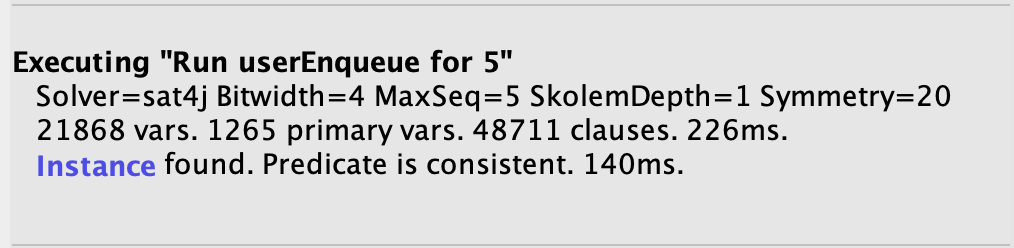
\includegraphics[width=0.6\textwidth]{Images/alloy/userenqueue.png}
    \caption{\label{fig:usernenqueuealloy}{todo}}
\end{figure}

\begin{figure}[h!]
    \centering
    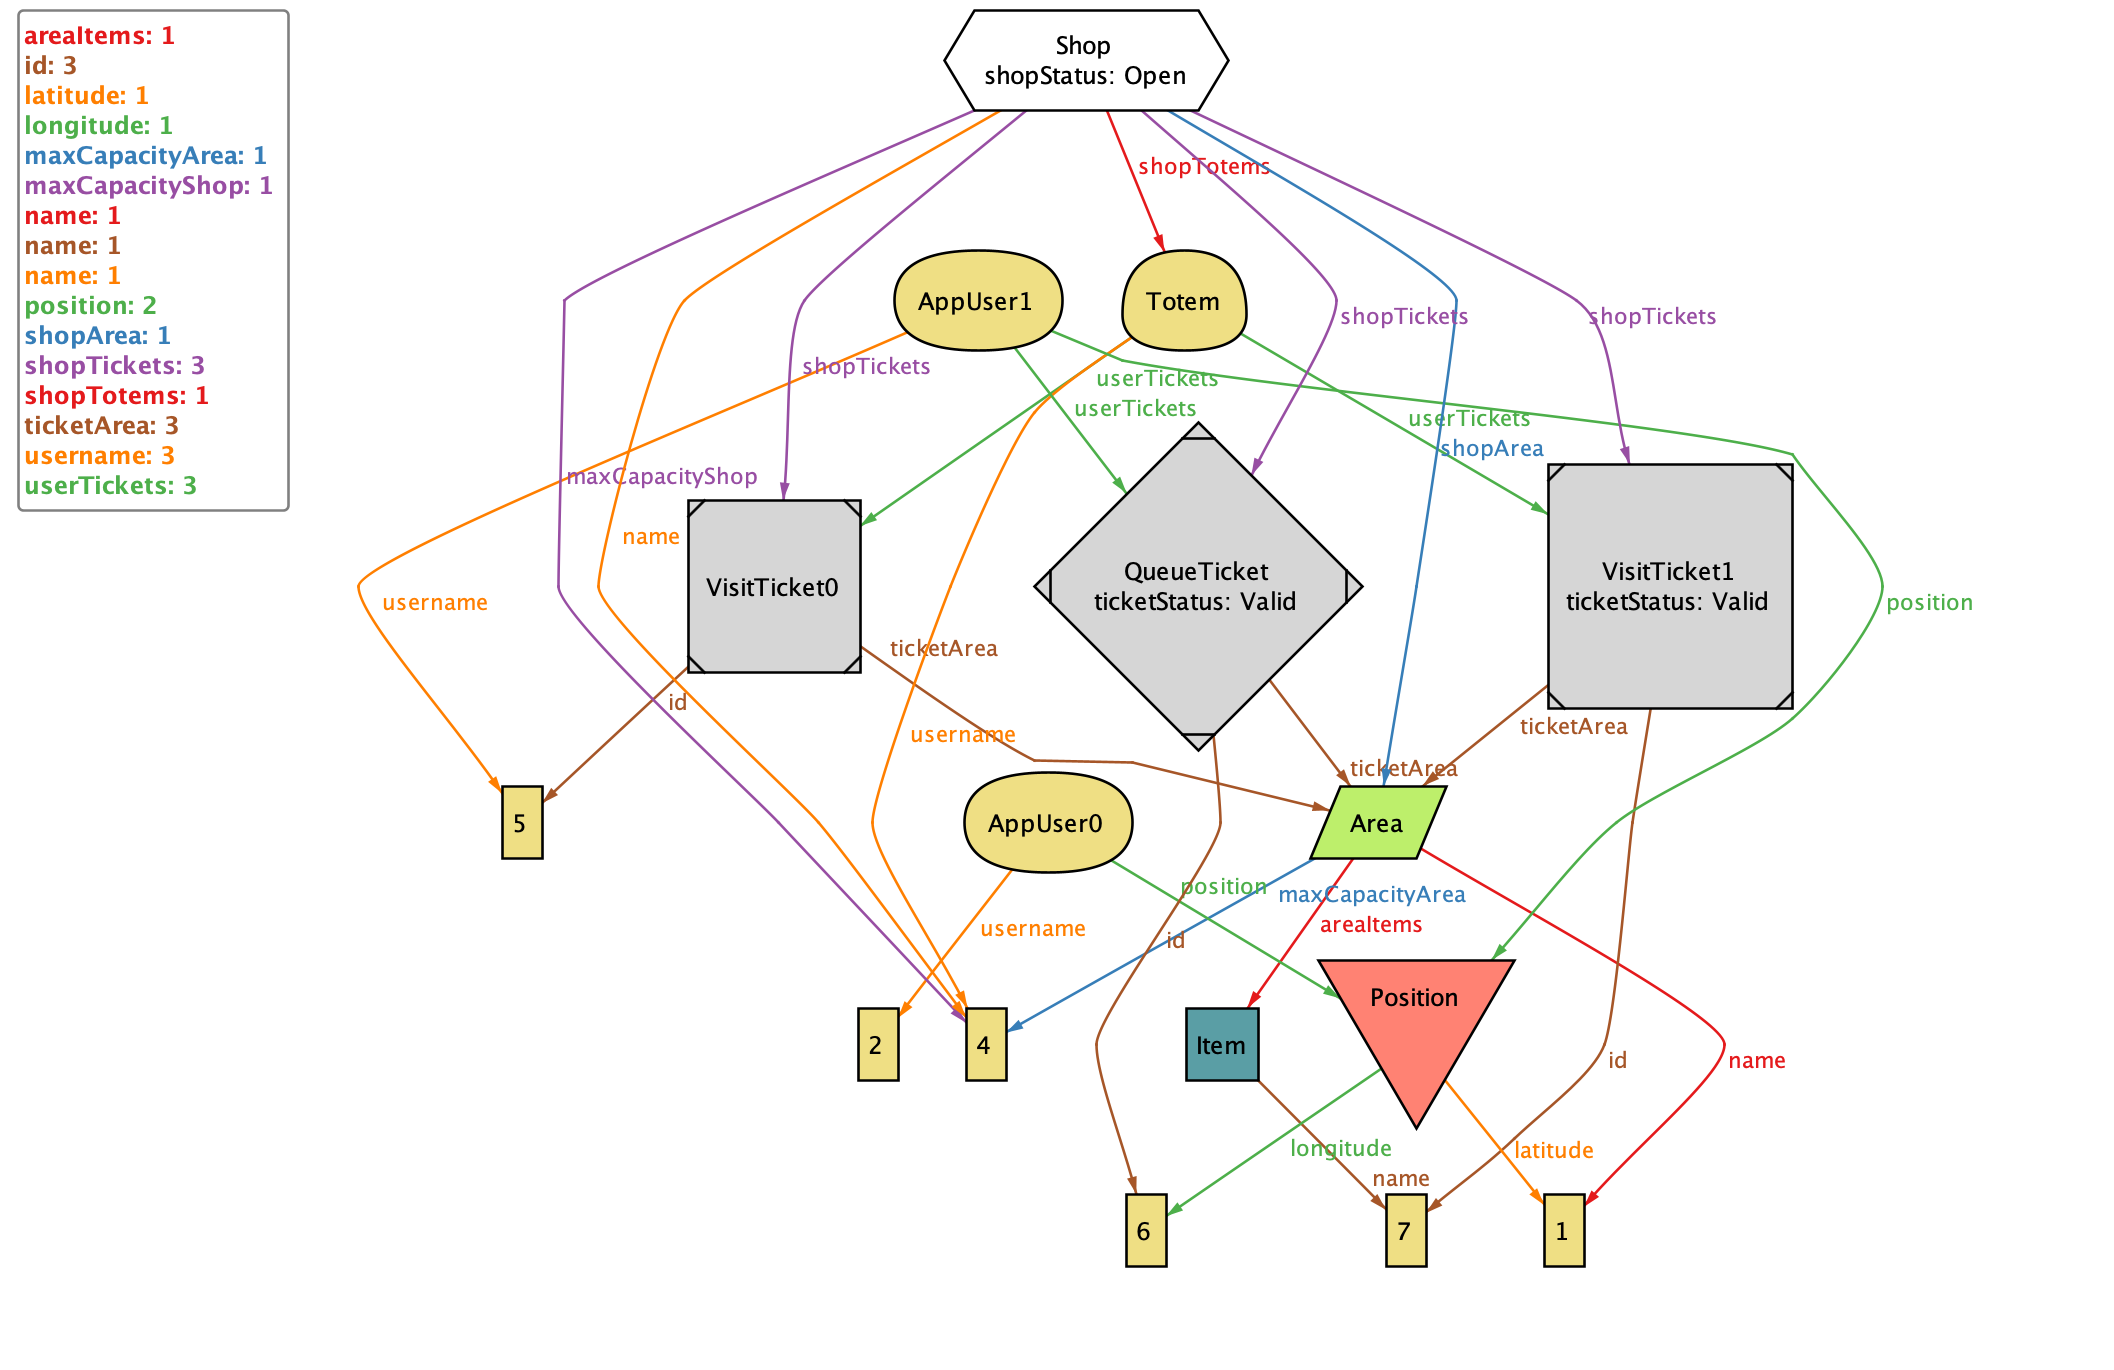
\includegraphics[width=\textwidth]{Images/alloy/alloymodel.png}
    \caption{\label{fig:alloymodel}{alloy model}}
\end{figure}

\FloatBarrier